\documentclass[12pt]{article}
\usepackage{graphicx}

\title{MATH4350 \\ Homework Assignment}
\author{Joel Savitz}
\date{Wednesday15 July 2020}

\begin{document}

\maketitle

\textbf{2a. The Babylonians generally determined the area of a circle
	by taking it as equal to $\frac{1}{12}$ the square of the circle’s
circumference. Show that this is equivalent to letting $\pi = 3$.}
\medskip

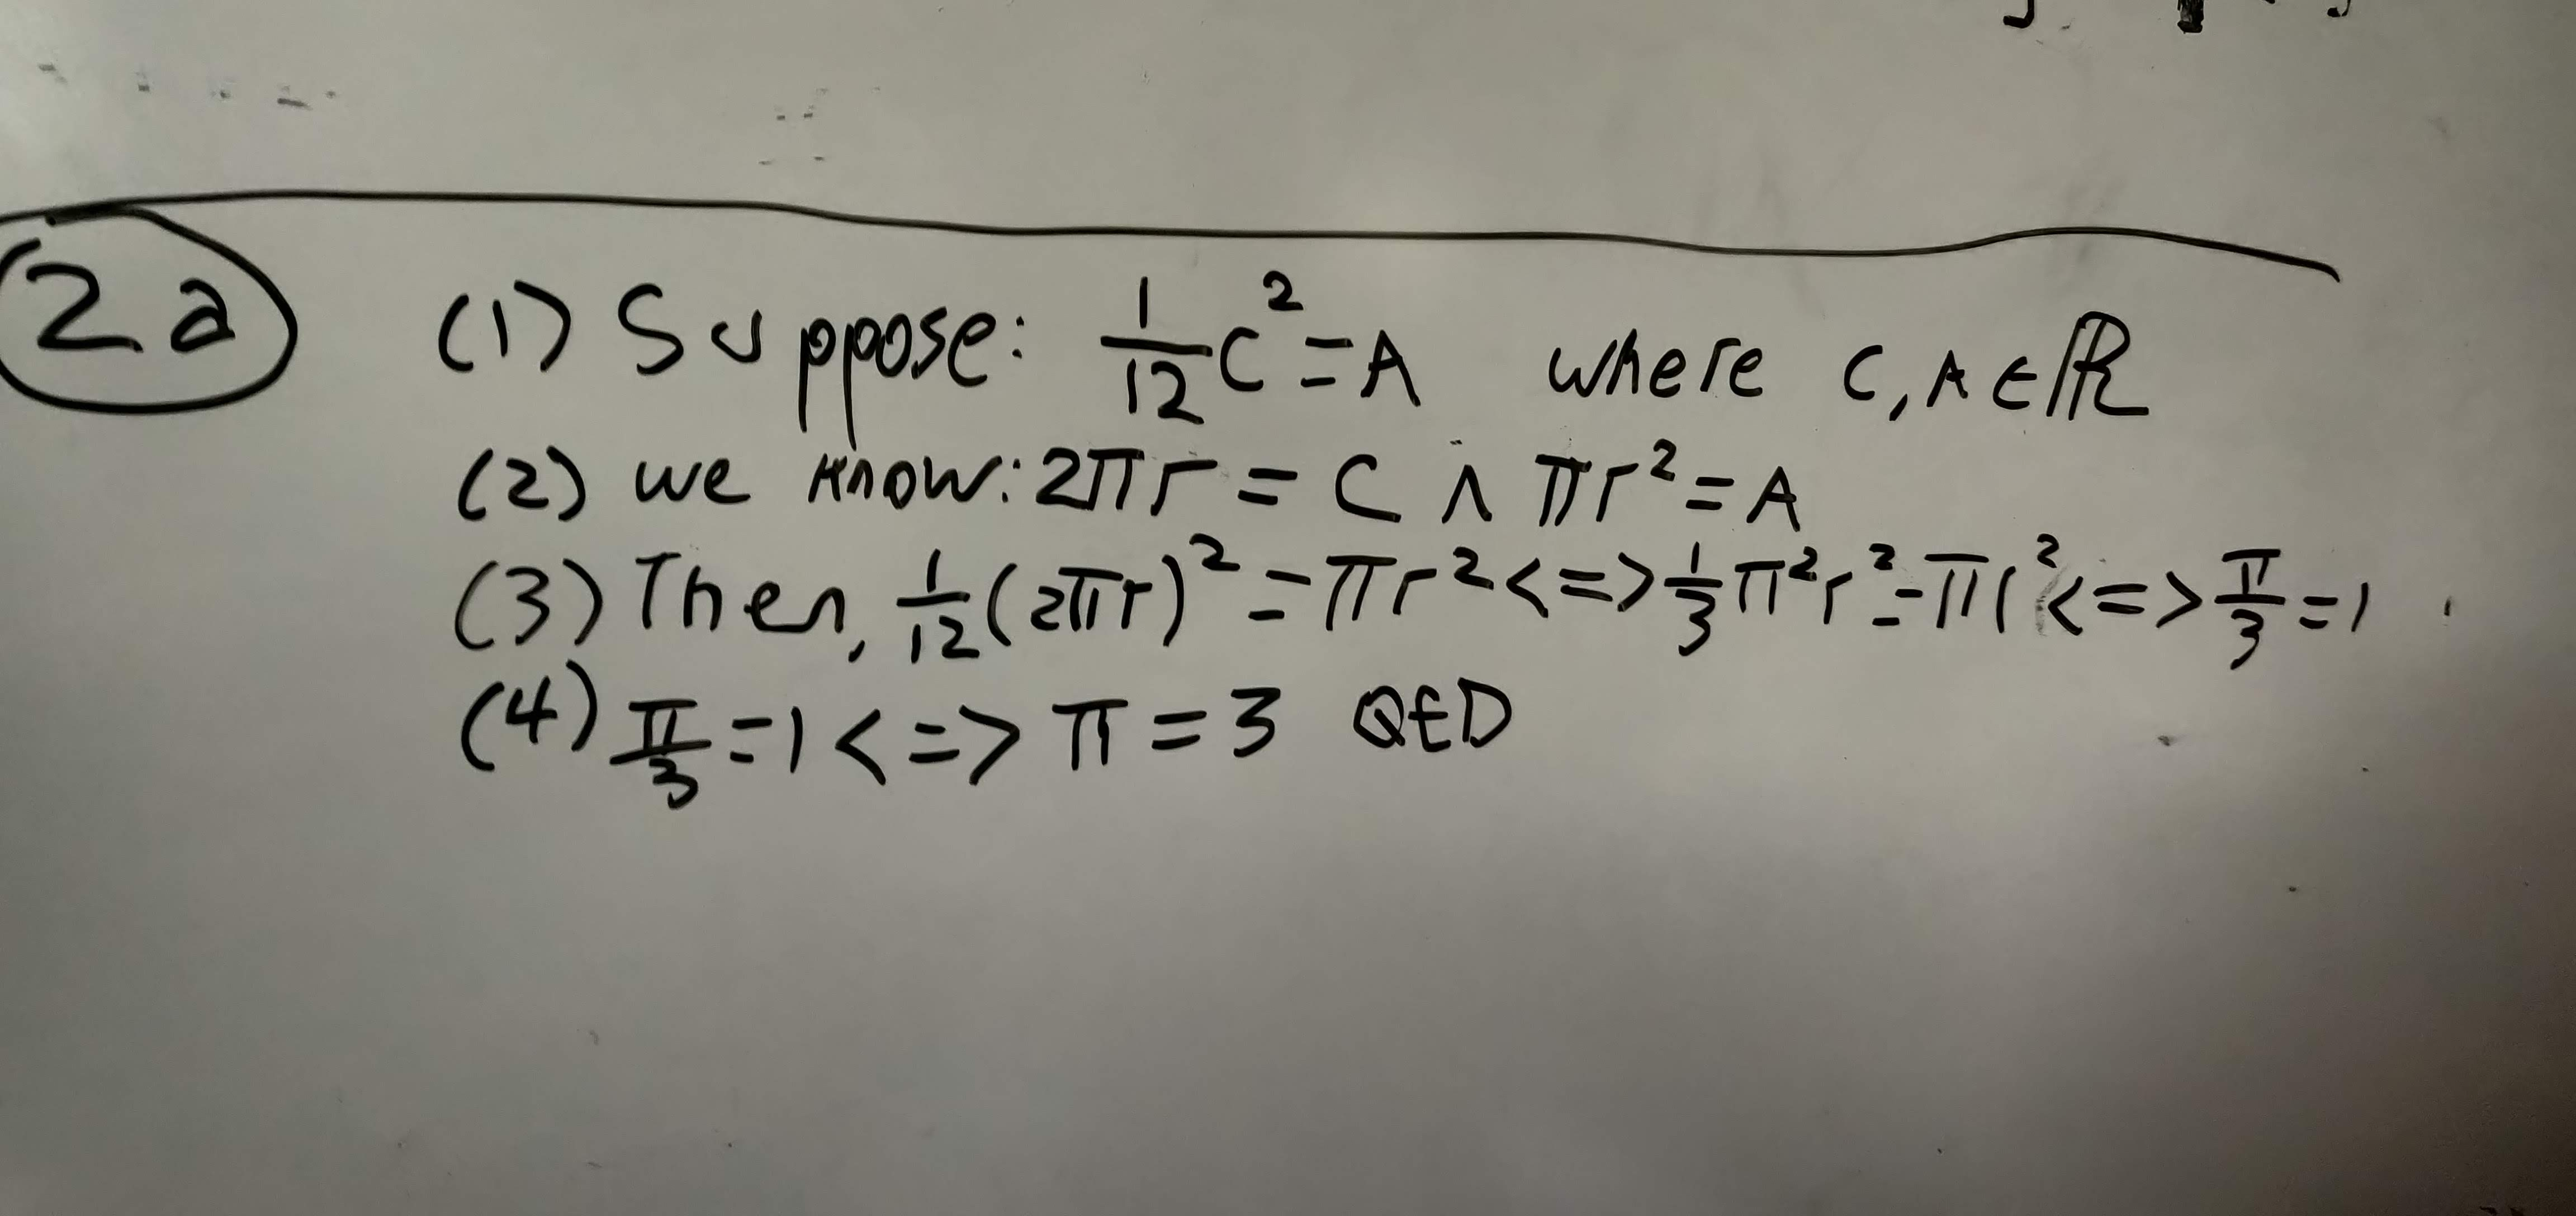
\includegraphics[scale=0.08]{2a.jpg}

\pagebreak
\textbf{2b. A Babylonian tablet excavated in 1936 asserts that when a more accurate determination of area is needed, the $\frac{1}{12}$ should be multiplied by 0;57,36, that is, by $\frac{24}{25}$. What value for $\pi$ does this correction factor yield?}
\medskip

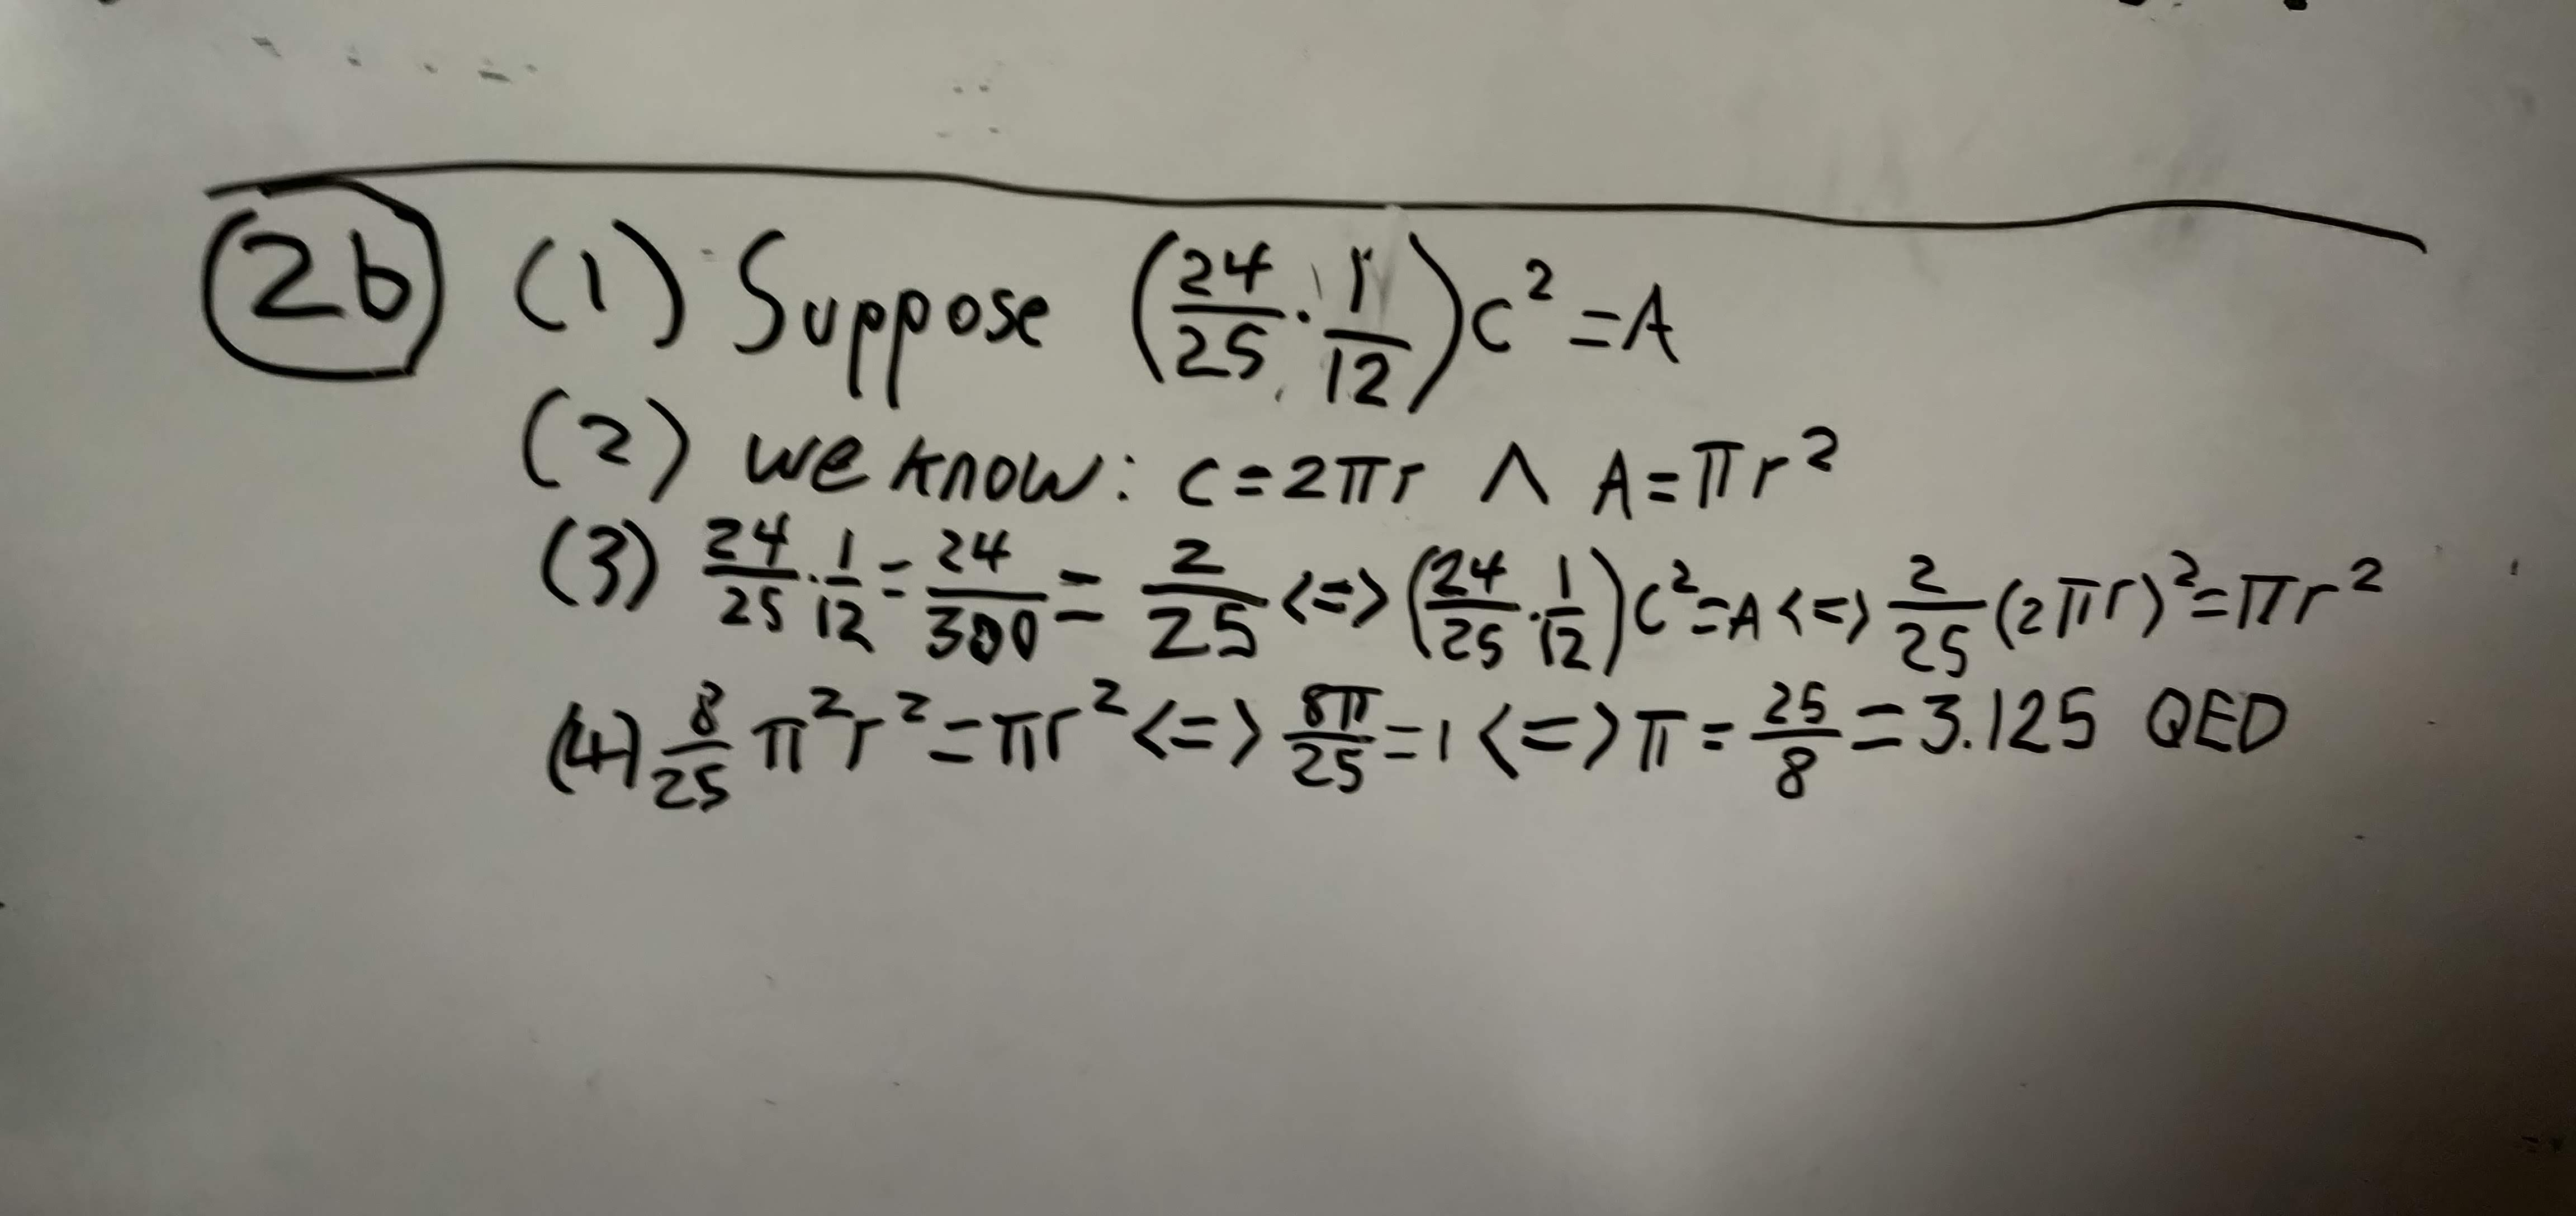
\includegraphics[scale=0.08]{2b.jpg}

\pagebreak
\textbf{3. Archimedes (about 287–212 B.C.) in his book \textit{Measurement of a Circle} stated: The area of a circle is to the square on its diameter as $11$ to $14$. Show that this geometric rule leads to $\frac{22}{7}$ for the value of $\pi$. }
\medskip

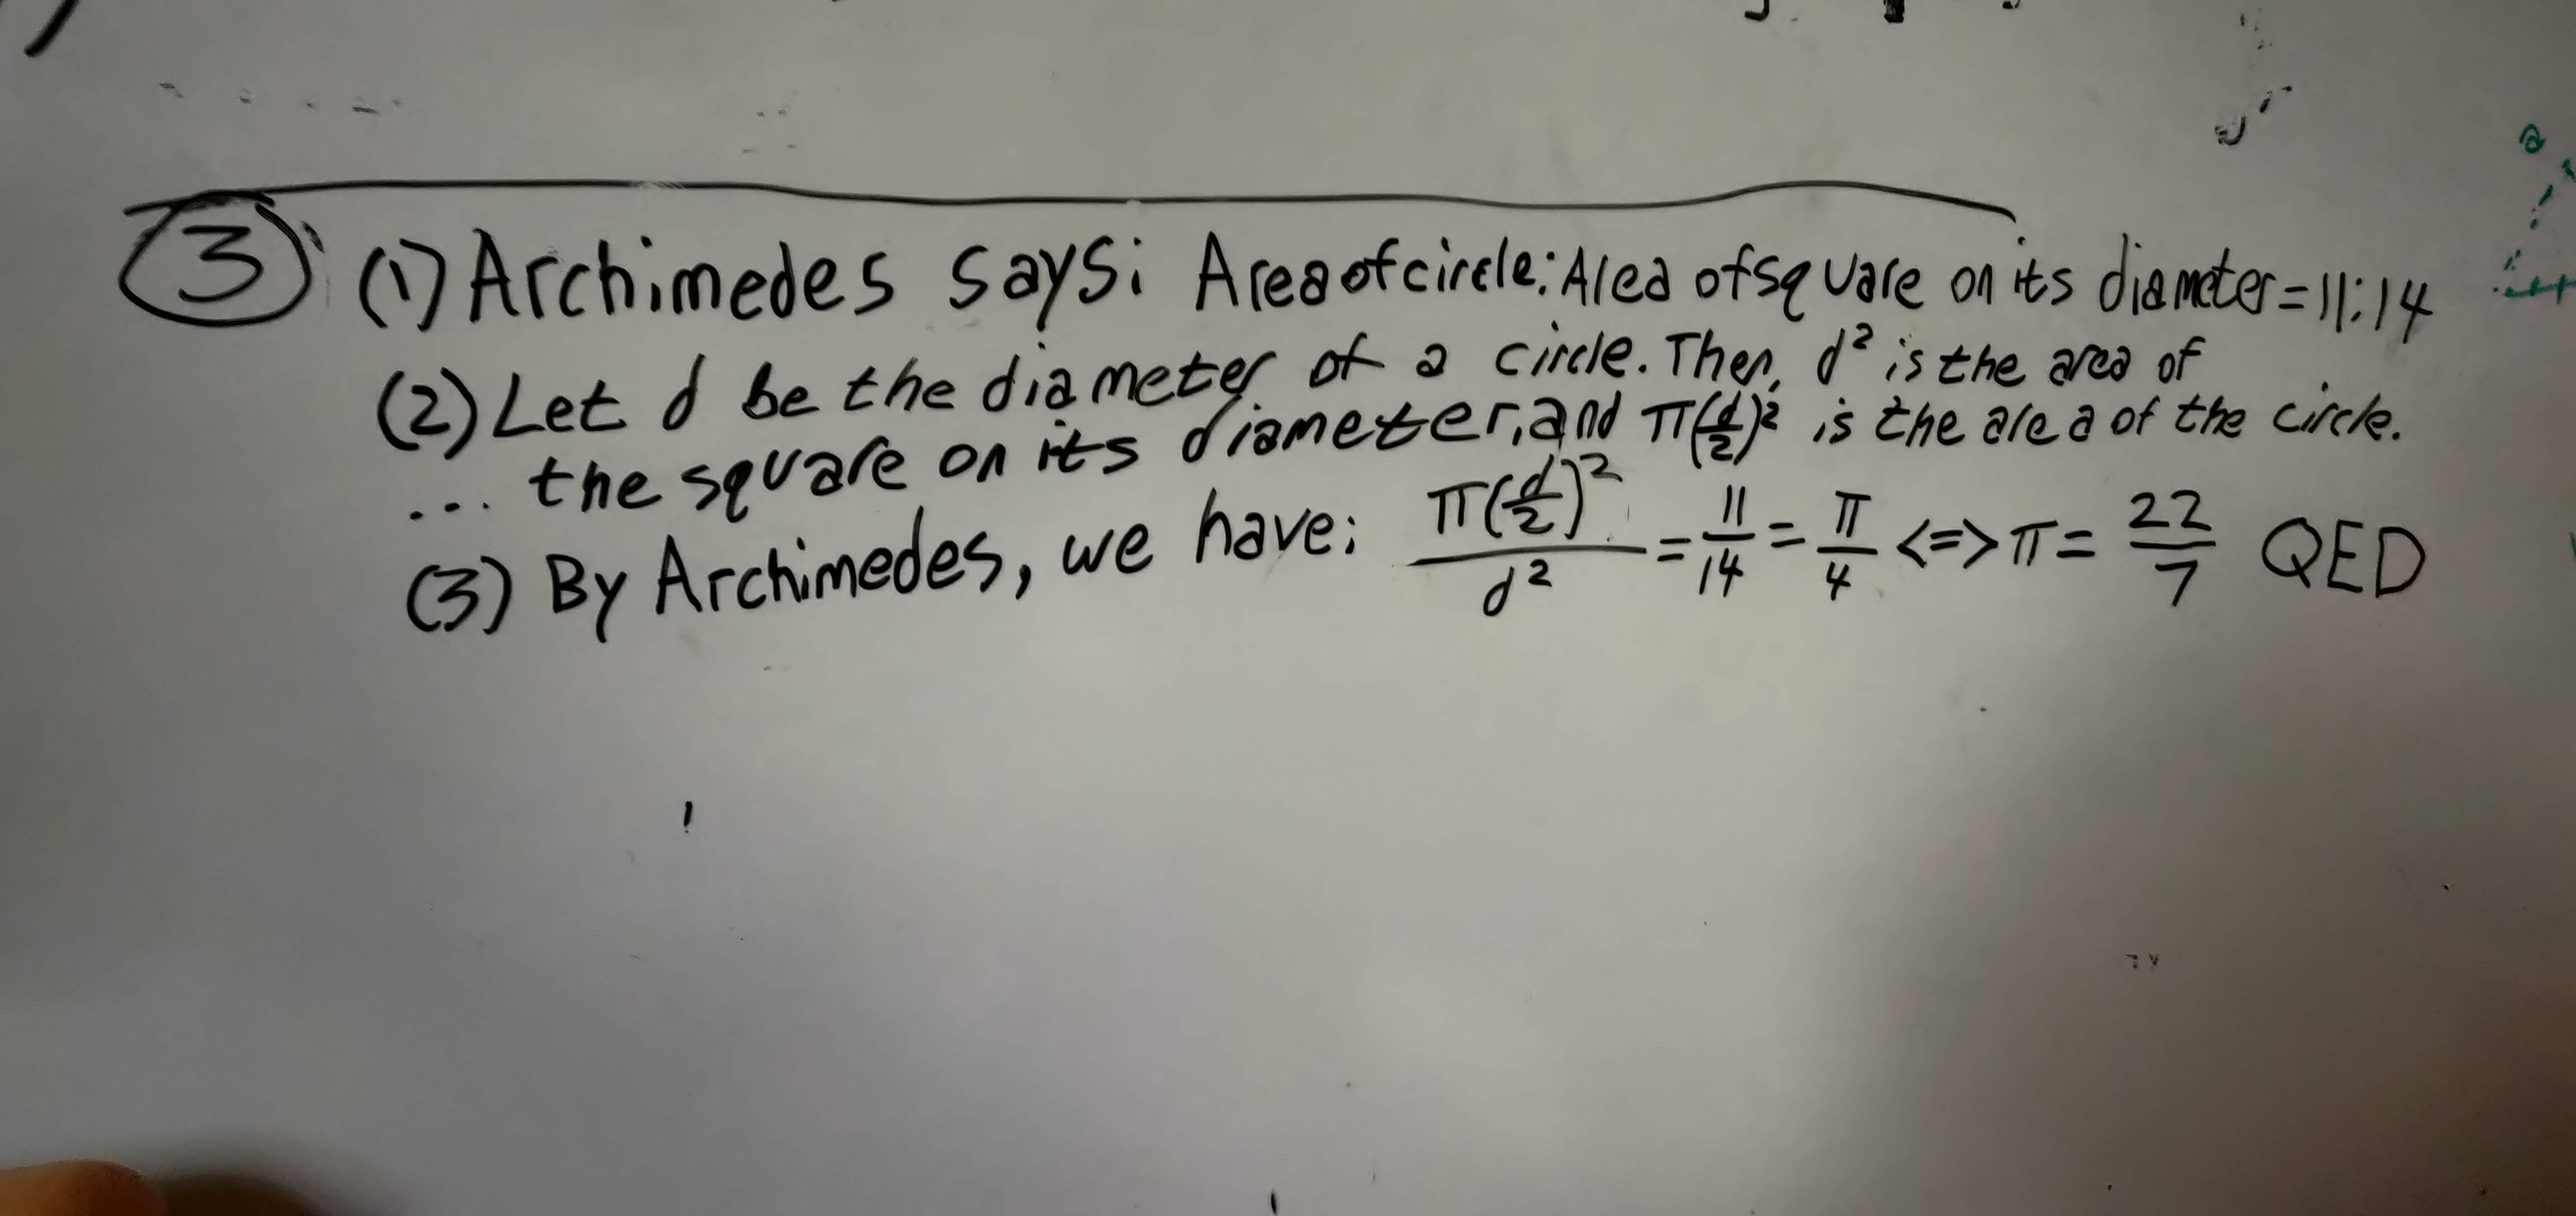
\includegraphics[scale=0.08]{3.jpg}

\pagebreak
\textbf{4. The sixth-century Hindu mathematician Aryabhata had the following procedure for finding the area of a circle: Half the circumference multiplied by half the diameter is the area of a circle. How accurate is this rule?}
\medskip

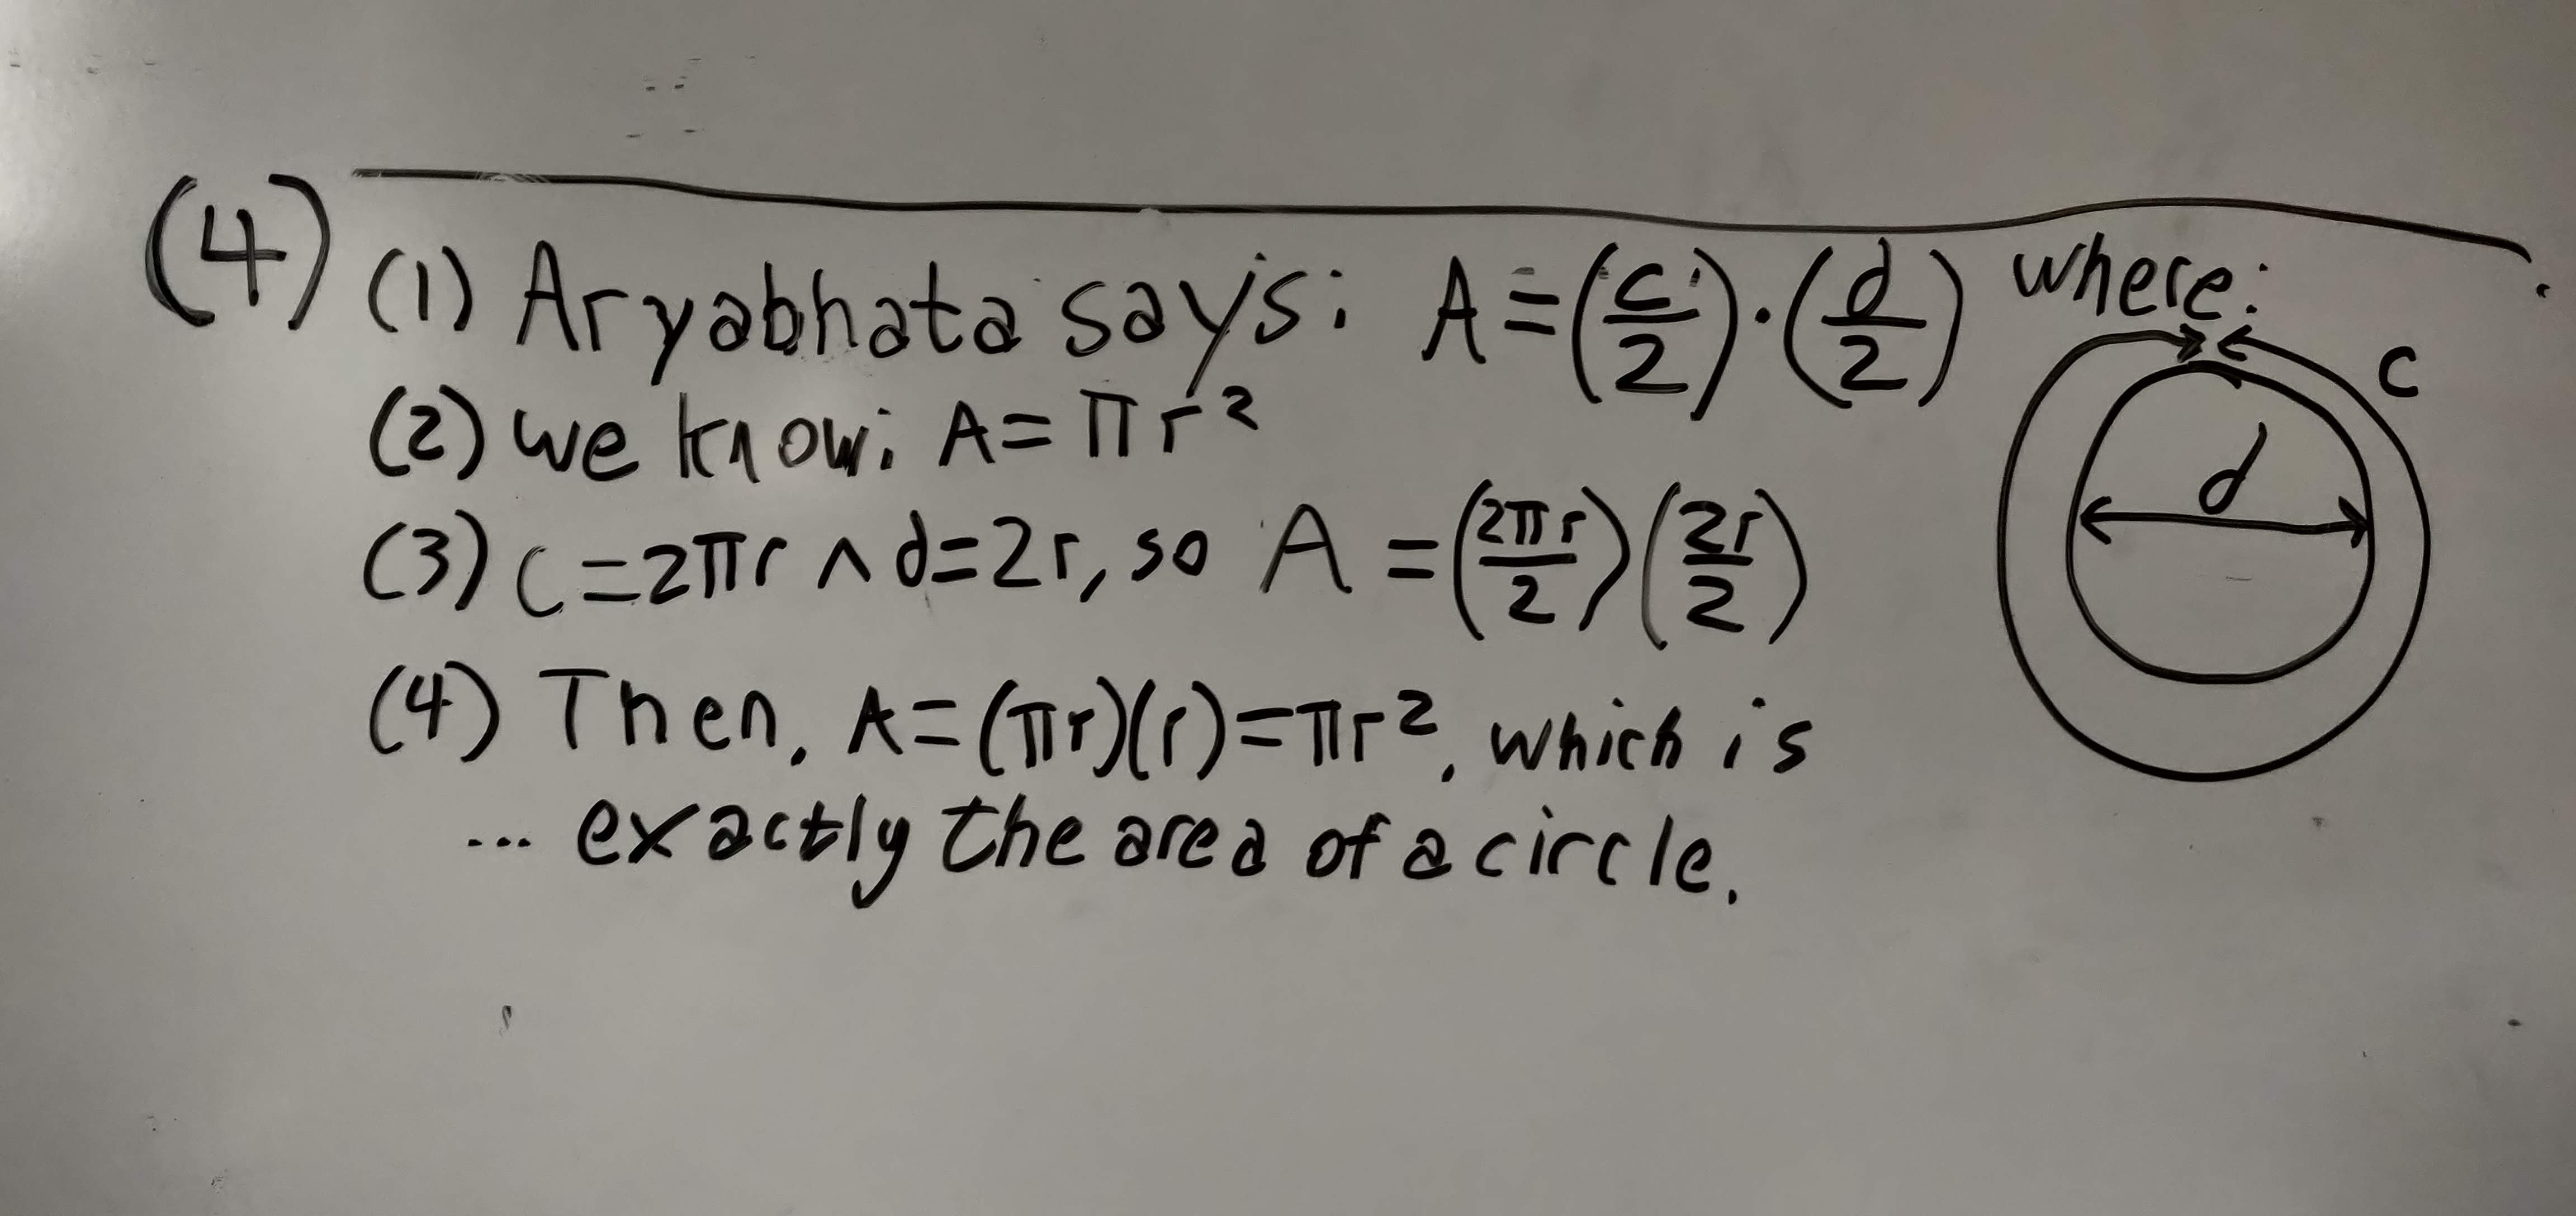
\includegraphics[scale=0.08]{4.jpg}

\end{document}
